\documentclass[a4paper,fleqn]{styles/cas-sc}

\usepackage[numbers]{natbib}
\usepackage[version=4]{mhchem}
\usepackage{amsmath}
\usepackage{booktabs}
\usepackage{graphicx}
\usepackage{subcaption}
\usepackage{siunitx}
\usepackage{tabularx}
\usepackage{xspace}
\usepackage{hyperref}
\usepackage{cleveref}

\graphicspath{{Figures/}}

\newcommand{\LiIon}{\ce{Li+}\xspace}
\newcommand{\NaIon}{\ce{Na+}\xspace}
\newcommand{\DES}{DES\xspace}
\newcommand{\TOPO}{TOPO\xspace}
\newcommand{\Smackover}{Smackover\xspace}
\newcommand{\Prommis}{PrOMMiS\xspace}
\newcommand{\IDAES}{IDAES\xspace}
\newcommand{\Dli}{D_{\mathrm{Li}}}
\newcommand{\Dna}{D_{\mathrm{Na}}}
\newcommand{\Slin}{S_{\mathrm{Li/Na}}}

\begin{document}

\let\WriteBookmarks\relax
\def\floatpagepagefraction{1}
\def\textpagefraction{.001}

\shorttitle{Produced-Water Lithium Extraction Case Study}
\shortauthors{Polley et al.}

\title[mode=title]{Rezaee-Calibrated Workflow for Produced-Water Lithium Extraction}

\author[1]{Tanner W. Polley}
\ead{tannerwpolley@gmail.com}

\begin{abstract}
Produced waters are attractive but chemically severe lithium resources because lithium can occur at tens to hundreds of milligrams per liter while sodium and divalent cations dominate the ionic background. This first-draft manuscript scaffolds a case study that treats a pretreated \Smackover source brine as a clean \LiIon/\NaIon extraction feed and uses the Rezaee hydrophobic \DES plus \TOPO chemistry as the active solvent basis. The current workflow converts Rezaee extraction evidence into distribution coefficients, evaluates a 523-row total-dissolved-solids, lithium-grade, and organic-to-aqueous screening matrix, and carries the resulting transfer variables into \Prommis/\IDAES process and costing artifacts. The manuscript intentionally distinguishes the calibrated distribution surrogate from a fully accepted direct reactive liquid--liquid ePC-SAFT split. It is written as a scaffold for a later complete paper once the high-\NaIon/\LiIon validation, staged contactor solution, and final techno-economic assumptions are fixed.
\end{abstract}

\begin{keywords}
lithium extraction\sep{}produced water\sep{}deep eutectic solvent\sep{}TOPO\sep{}ePC-SAFT\sep{}PrOMMiS\sep{}IDAES
\end{keywords}

\maketitle

\section{Introduction}
\label{sec:introduction}

Direct lithium extraction from unconventional brines requires a thermodynamic and process model that can separate the lithium recovery question from the brine-severity question. Produced waters are especially relevant because they can combine high total dissolved solids, large sodium excess, and measurable lithium concentrations with existing water-handling infrastructure. Those same features make the separation problem hard: the extraction solvent sees a high-ionic-strength feed, and any direct solvent model must either include divalent competition explicitly or define a pretreated feed boundary.

This manuscript frames the case study around a pretreated \Smackover \LiIon/\NaIon stream. The current presentation and analysis chain does not use the older HBTA/TOPO solvent-selection lane as the active case-study basis. Instead, it uses the hydrophobic \DES plus \TOPO extraction chemistry reported by Rezaee and co-workers as the solvent evidence base \cite{Rezaee2025RSM,Rezaee2026PCSASFTSI}. The resulting contribution is not a new extraction solvent, but a traceable engineering workflow that connects literature extraction data, ePC-SAFT-facing parameter artifacts, a distribution-coefficient surrogate, and downstream \Prommis/\IDAES process screening.

The first-draft paper is organized around four questions:
\begin{enumerate}
    \item Which produced-water composition should be used as the clean \LiIon/\NaIon case-study basis?
    \item How should Rezaee extraction data be converted into process-facing distribution coefficients without claiming unsupported direct reactive-LLE closure?
    \item What range of lithium recovery, sodium co-extraction, selectivity, and transfer coefficients is produced by the current calibrated screening matrix?
    \item Which assumptions must be promoted before the \Prommis/\IDAES costing layer can be interpreted as a final techno-economic analysis?
\end{enumerate}

\section{Source Basis and Case Definition}
\label{sec:source-basis}

\subsection{Produced-water screening}

The project screening table compares common brine classes by lithium concentration, total dissolved solids, sodium load, and divalent-cation interference. The active candidate basis is a \Smackover produced-water row because it combines a high lithium grade with a hypersaline operating envelope. The current source table ranks the high-observed \Smackover case at \SI{252}{mg/L} lithium and the MS-2 base case at \SI{168}{mg/L} lithium. The MS-2 base row is used as the nominal process-screening feed because it has a complete clean \LiIon/\NaIon handoff row in the current artifacts.

\begin{figure}
    \centering
    \begin{subfigure}{0.48\linewidth}
        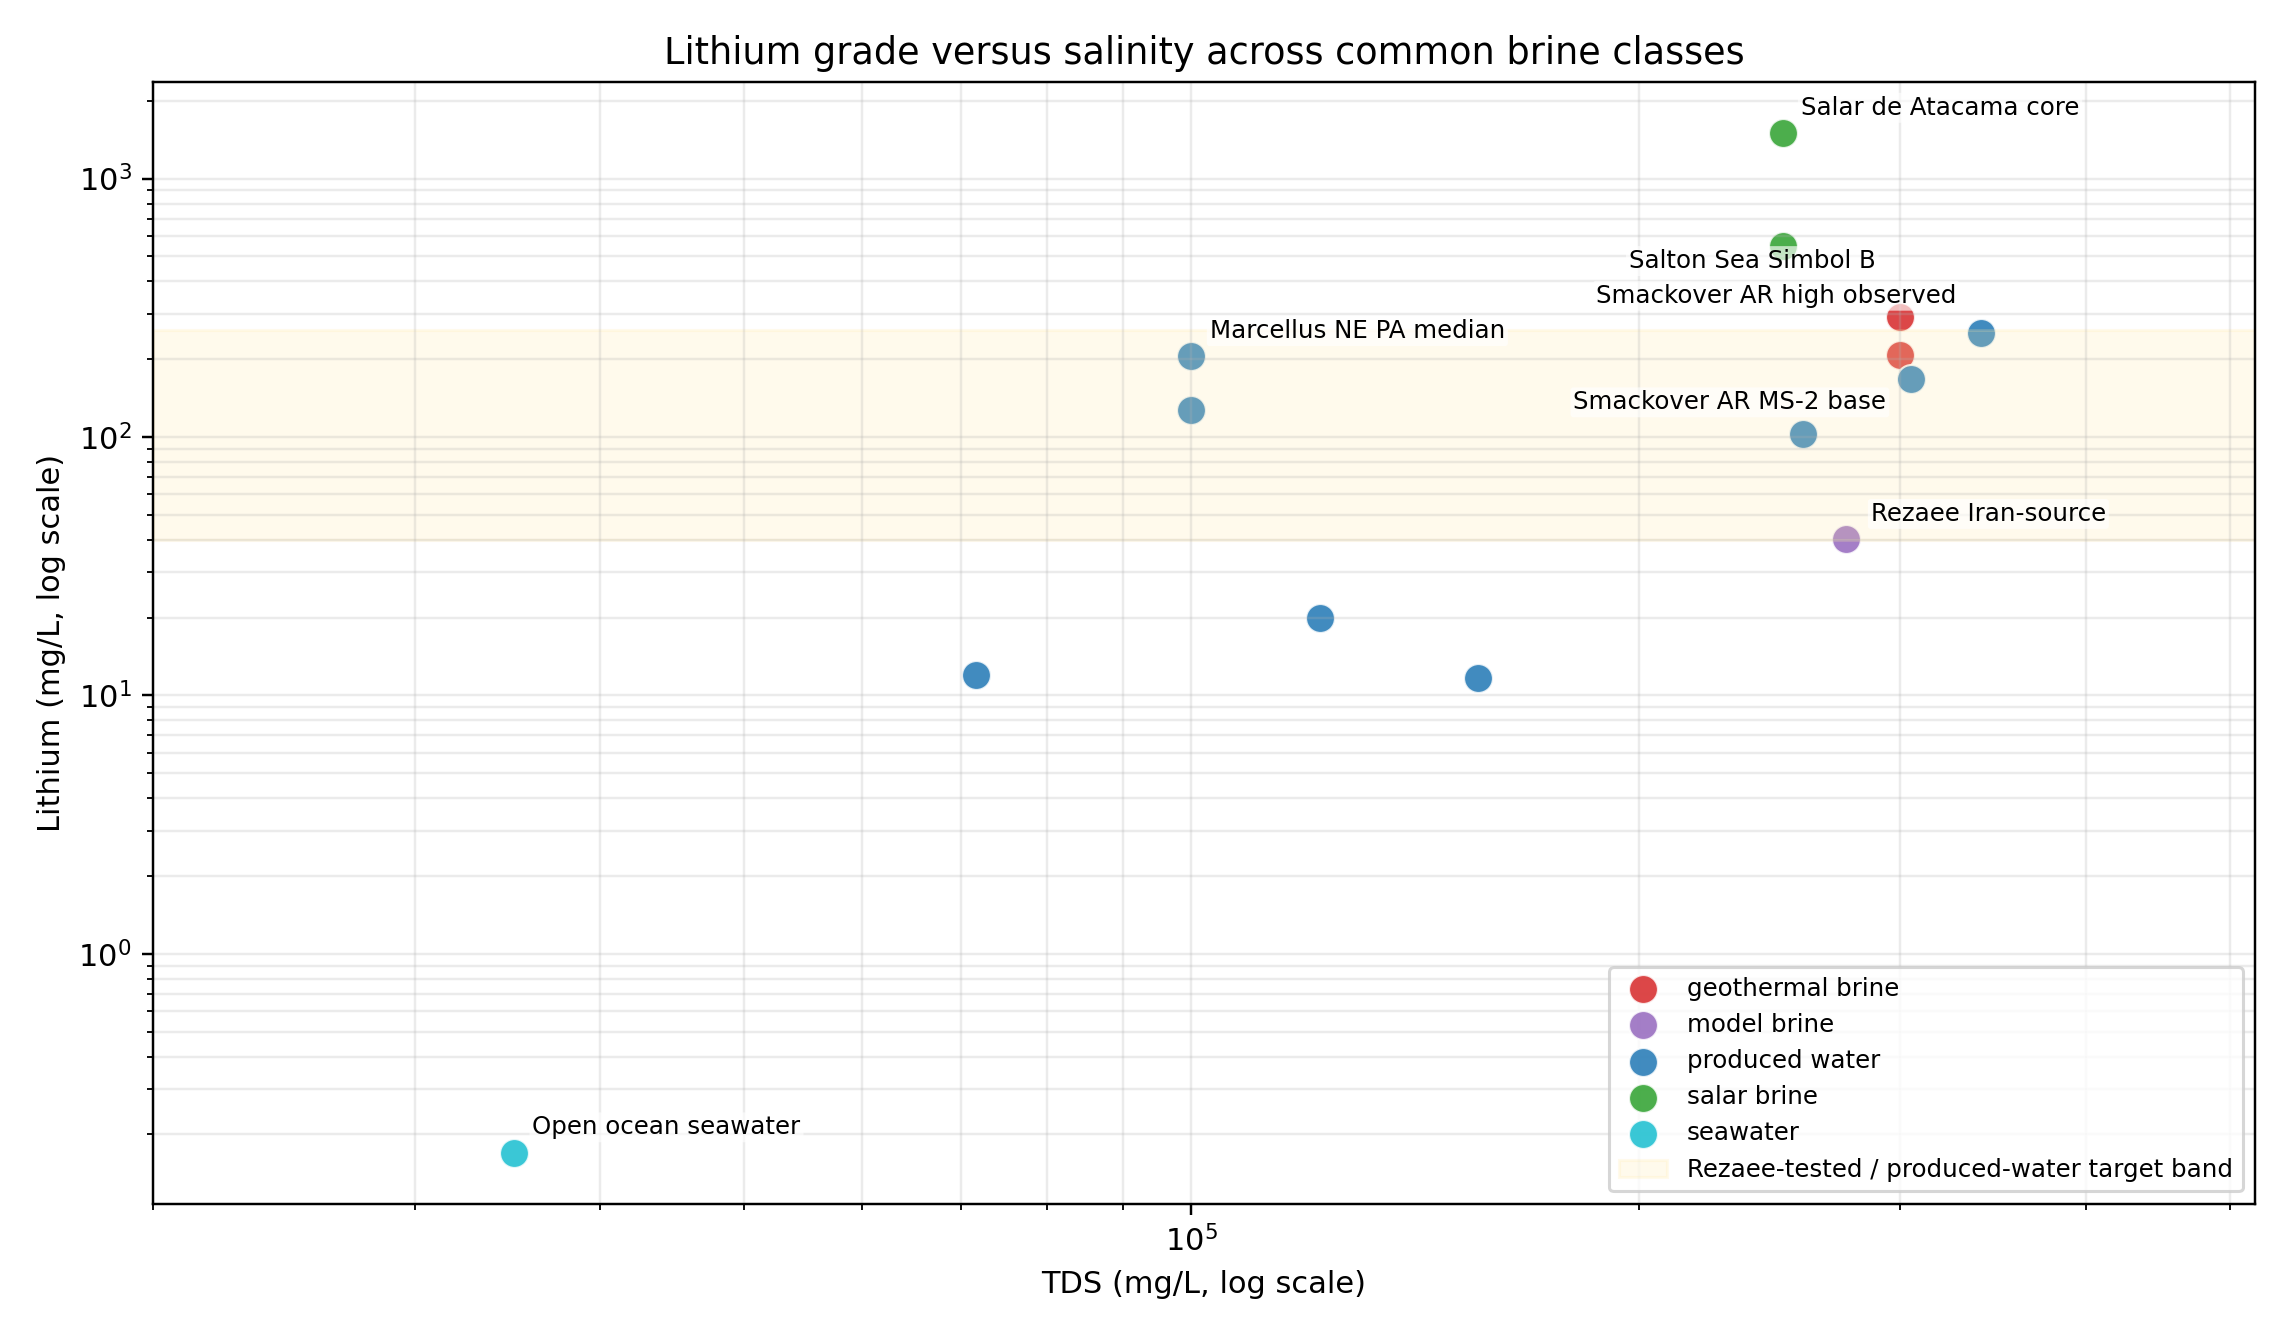
\includegraphics[width=\linewidth]{brine_li_tds_scatter.png}
        \caption{Lithium grade versus salinity for screened brine classes.}
        \label{fig:brine-scatter}
    \end{subfigure}
    \hfill
    \begin{subfigure}{0.48\linewidth}
        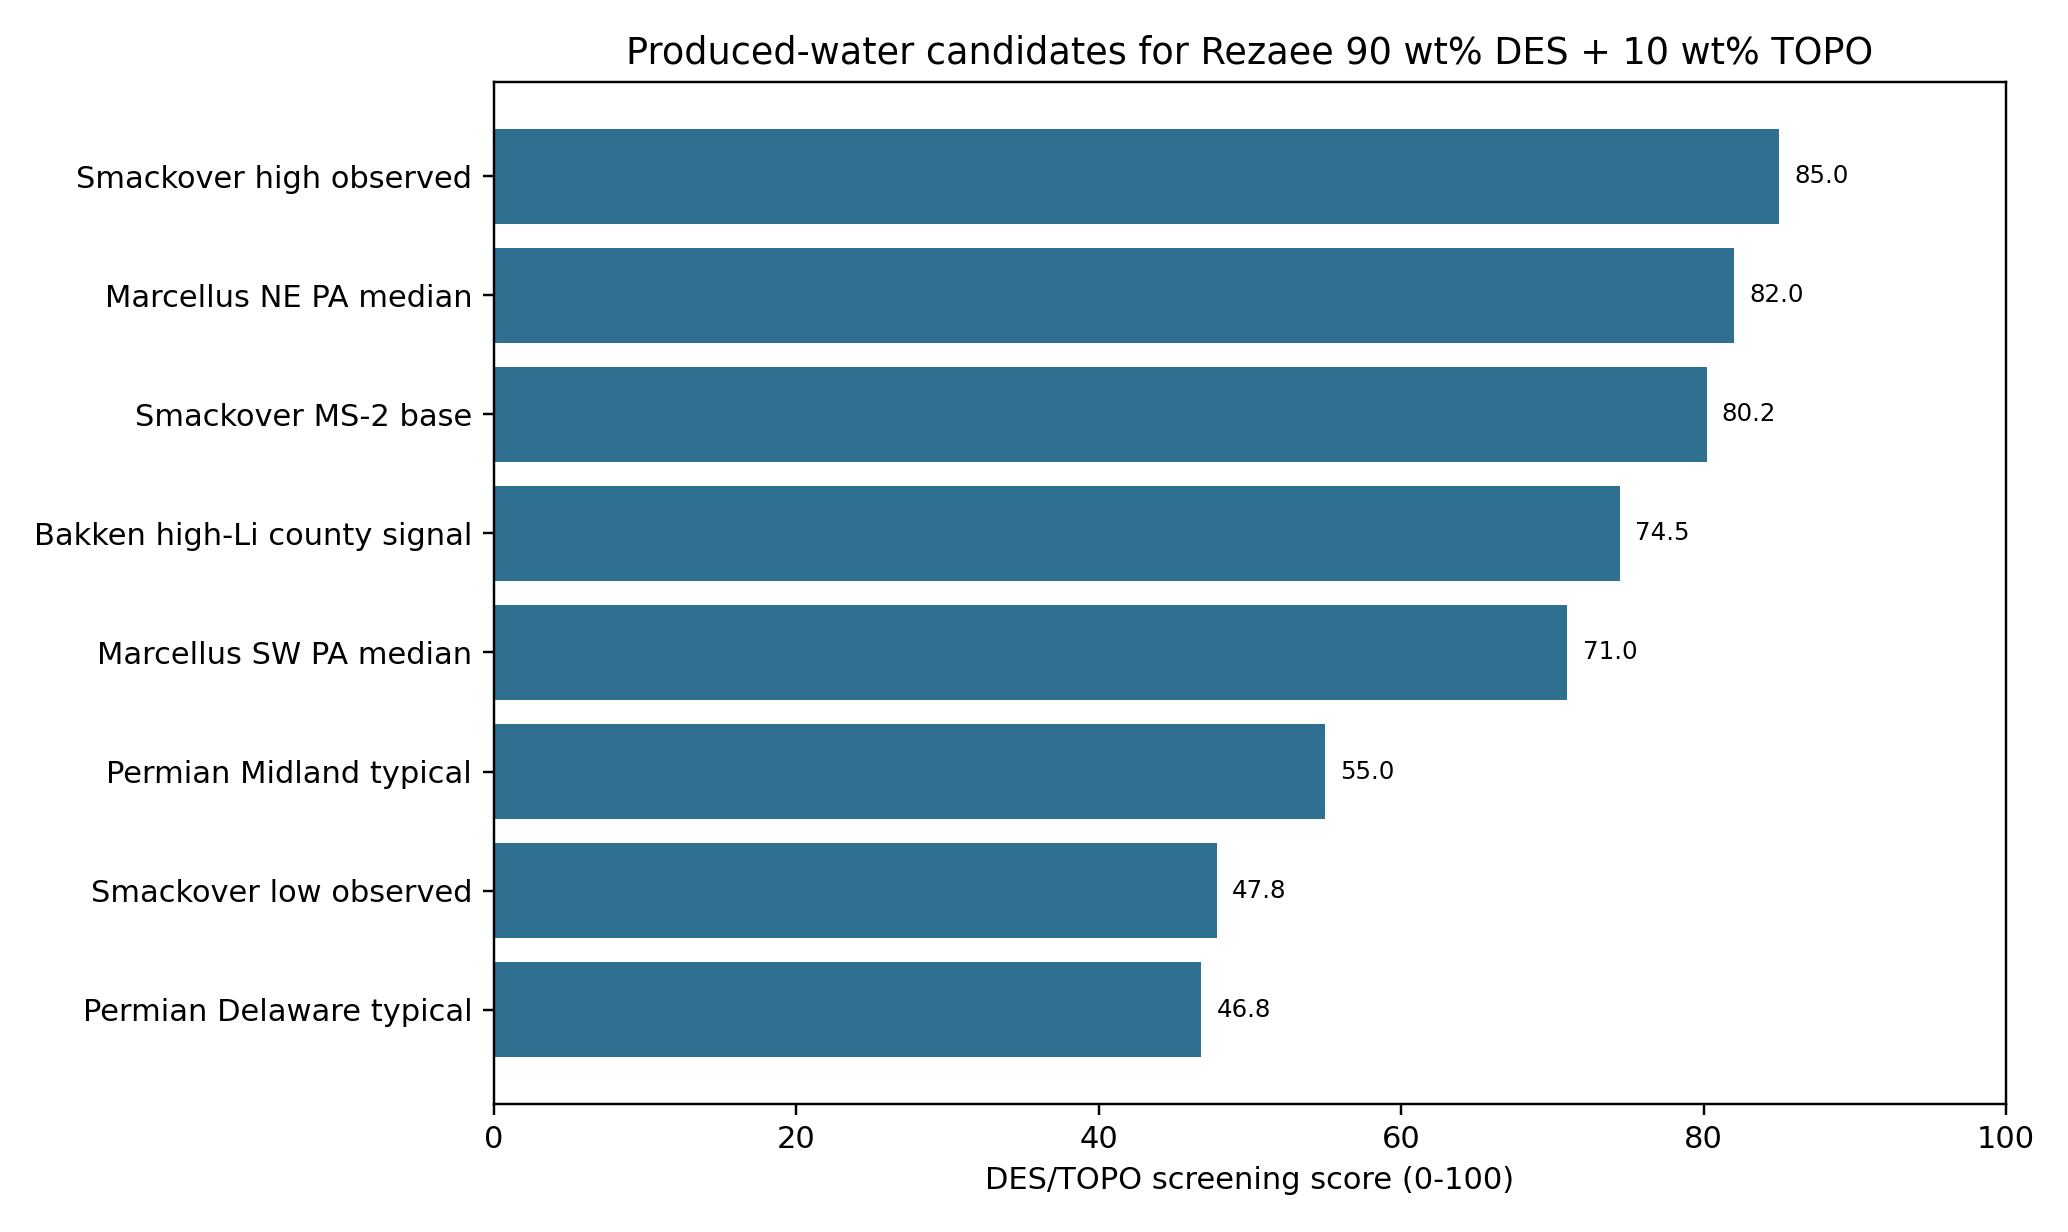
\includegraphics[width=\linewidth]{produced_water_candidate_scores.png}
        \caption{Produced-water candidate ranking for the Rezaee solvent basis.}
        \label{fig:candidate-scores}
    \end{subfigure}
    \caption{Composition screening figures copied from the project analysis artifacts. The score is a screening metric, not a resource estimate.}
    \label{fig:composition-screening}
\end{figure}

\subsection{Pretreatment boundary}

The process basis assumes that divalent cations are removed before solvent extraction. Calcium, magnesium, strontium, and barium are therefore pretreatment and costing variables, not competitive species in the current Rezaee \DES/\TOPO extraction surrogate. This boundary is essential because the Rezaee calibration basis is strongest for a clean \LiIon/\NaIon transfer model, while the raw produced-water composition contains additional ions that would require a larger validated reactive liquid--liquid model.

\begin{figure}
    \centering
    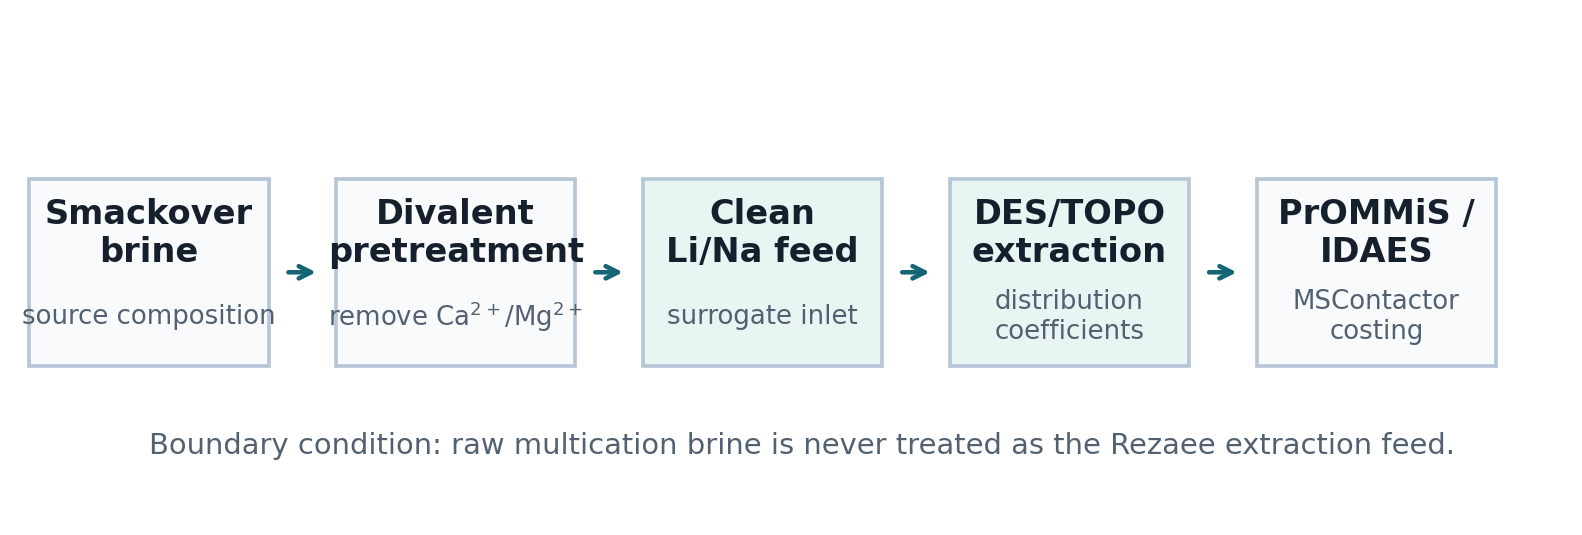
\includegraphics[width=0.85\linewidth]{process_bridge_diagram.png}
    \caption{Active case-study boundary from raw \Smackover brine to pretreated \LiIon/\NaIon extraction feed and \Prommis/\IDAES handoff.}
    \label{fig:process-boundary}
\end{figure}

\section{Thermodynamic Surrogate Method}
\label{sec:method}

The current case study uses a calibrated distribution surrogate rather than a direct claim of complete reactive ePC-SAFT LLE closure. Rezaee extraction responses are translated into species distribution coefficients using the organic-to-aqueous phase ratio,
\begin{equation}
    D_i = \frac{E_i/(100-E_i)}{O/A},
    \label{eq:distribution}
\end{equation}
where $E_i$ is the single-stage extraction percentage of species $i$ and $O/A$ is the organic-to-aqueous mass or phase-ratio basis used by the screening row. The lithium-to-sodium selectivity is then
\begin{equation}
    \Slin = \frac{\Dli}{\Dna}.
    \label{eq:selectivity}
\end{equation}

The current implementation fits lightweight response surfaces in log-distribution space and evaluates a 523-row screening matrix. The active input variables are total dissolved solids, lithium feed concentration, and organic-to-aqueous ratio at fixed Rezaee chemistry settings. The current scaffold should be updated later with the exact regression form, cross-validation diagnostics, and uncertainty propagation once the final surrogate file is locked.

\begin{figure}
    \centering
    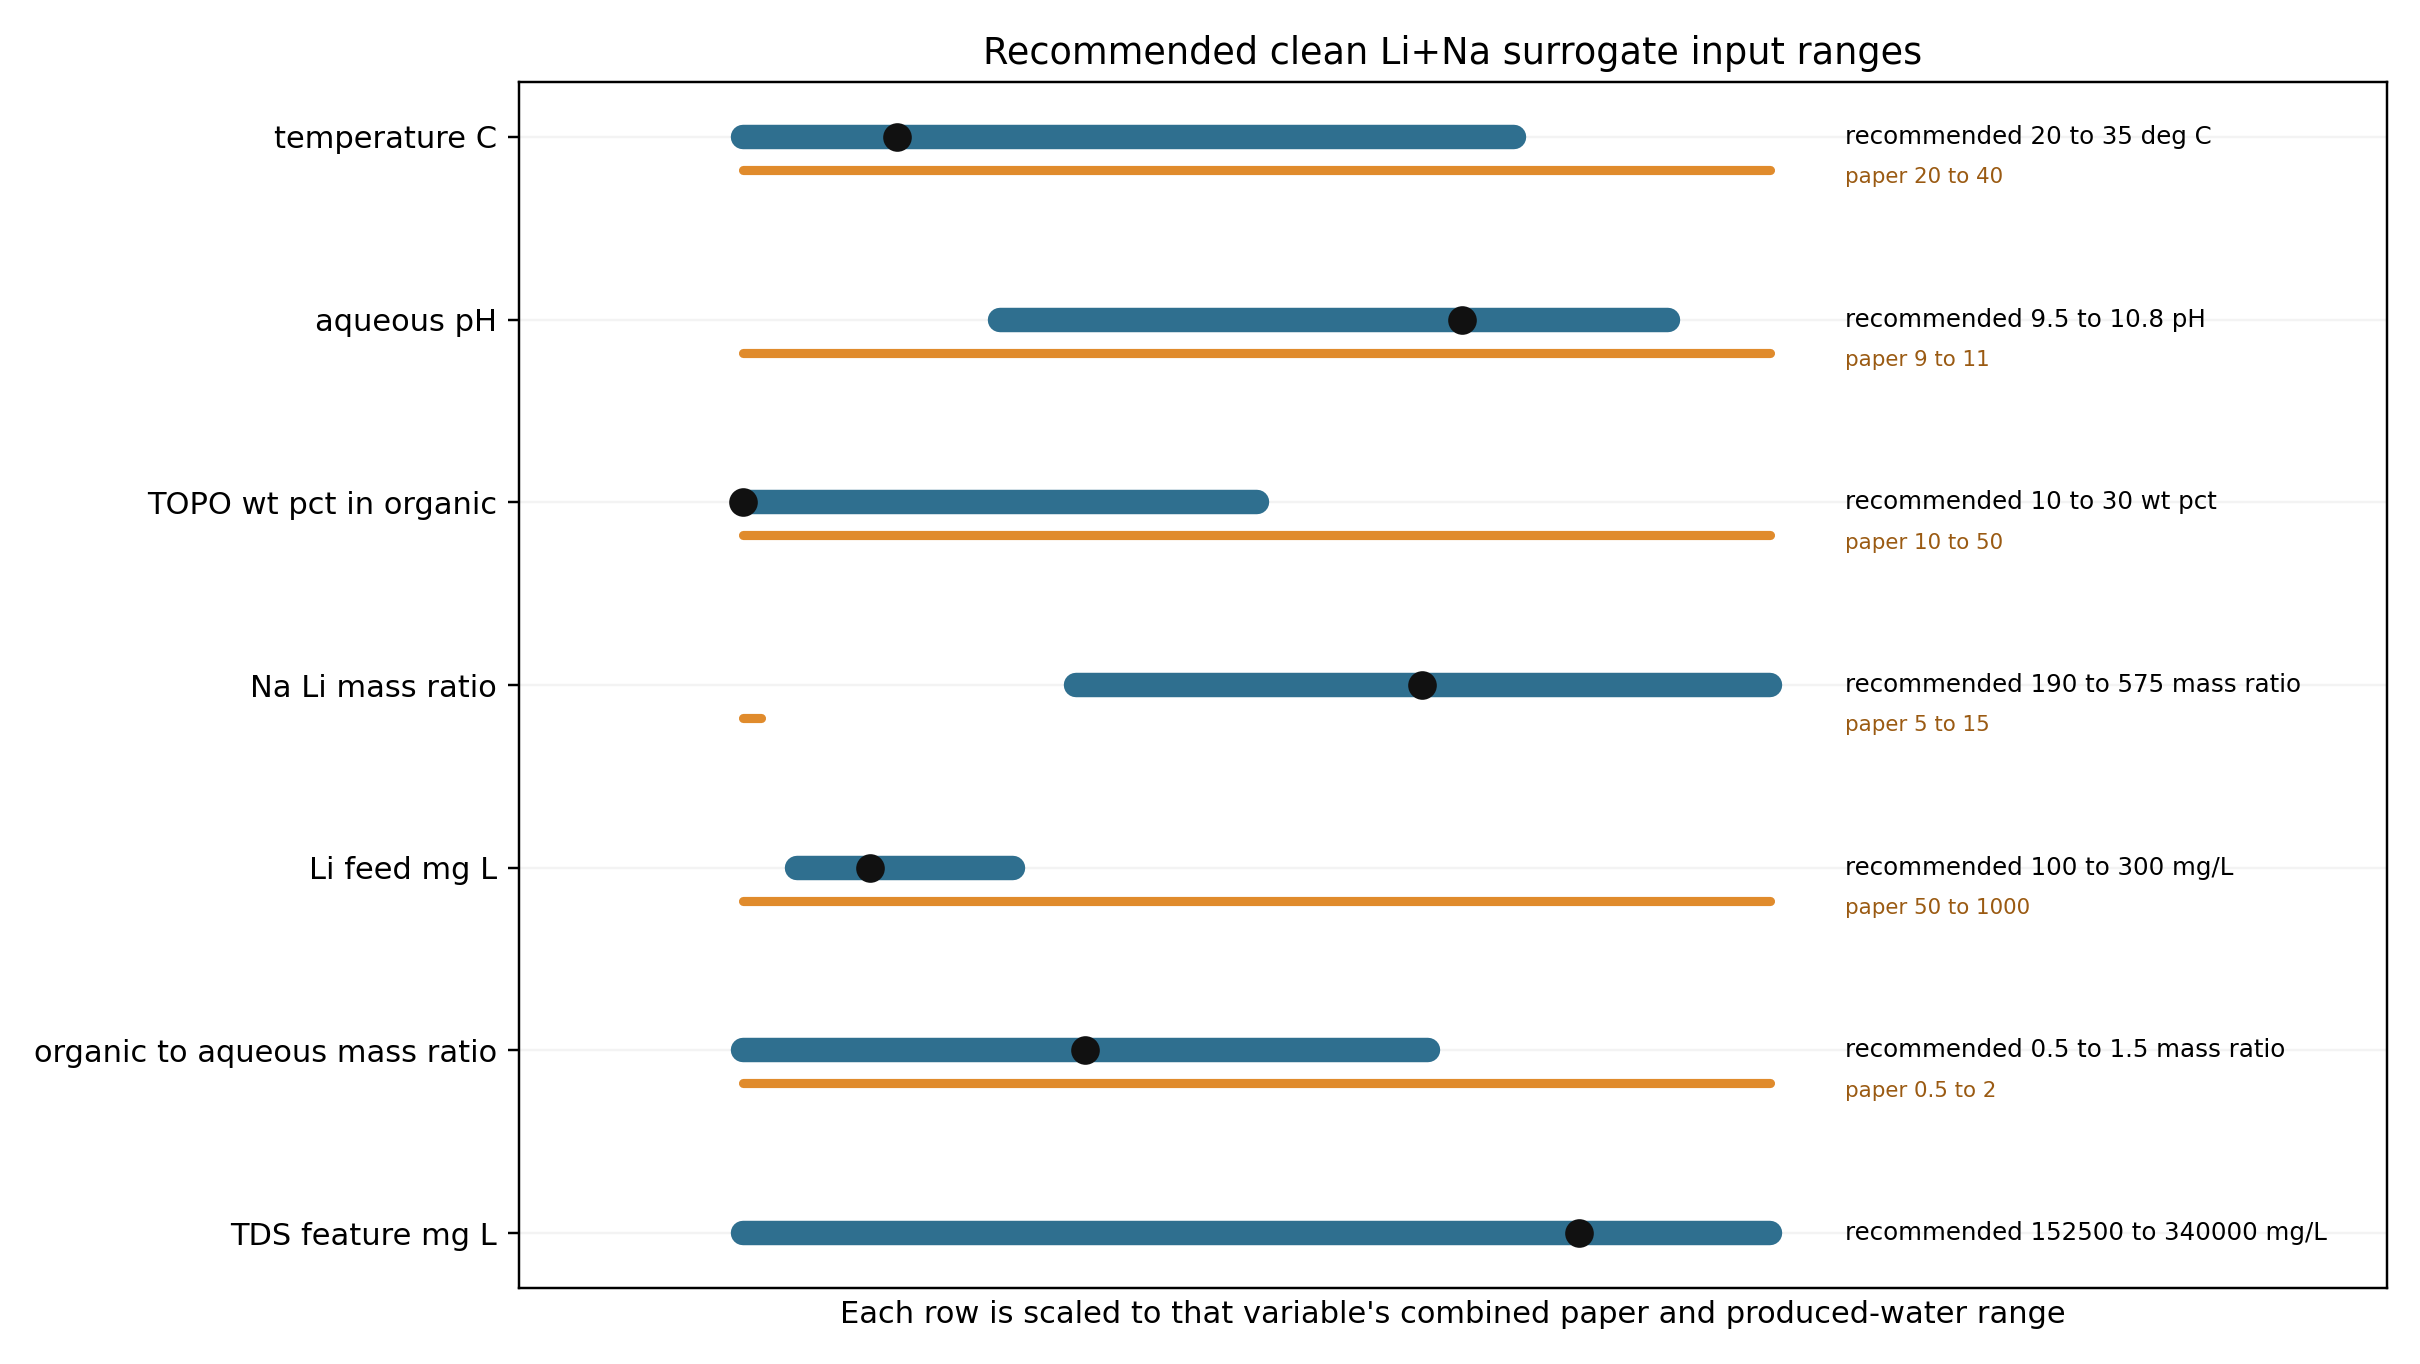
\includegraphics[width=0.86\linewidth]{rezaee_surrogate_input_ranges.png}
    \caption{Recommended clean \LiIon/\NaIon surrogate input ranges used to create the current screening matrix.}
    \label{fig:input-ranges}
\end{figure}

\subsection{ePC-SAFT role}

The Rezaee supporting information provides organic pseudo-component, binary-interaction, reaction-constant, and density evidence that is useful for an ePC-SAFT-facing model. In the current case study, those inputs are used as traceable thermodynamic evidence and as a package-facing bridge. The direct ePC-SAFT reactive-LLE solve remains a validation target, not the accepted physical split used for the current process deck. This distinction is preserved in the manuscript because it controls how strongly the process and cost results may be interpreted.

\section{Produced-Water Screening Results}
\label{sec:screening-results}

The calibrated surrogate returns finite outputs over the current produced-water screening matrix. The generated matrix spans approximately \SIrange{30.2}{61.4}{\percent} one-stage lithium extraction and \SIrange{2.7}{9.8}{\percent} sodium extraction. The nominal MS-2 clean \Smackover row gives \SI{50.66}{\percent} one-stage lithium extraction and \SI{5.67}{\percent} sodium extraction at $O/A=1.0$, corresponding to $\Dli=1.0267$, $\Dna=0.0601$, and $\Slin=17.09$.

\begin{figure}
    \centering
    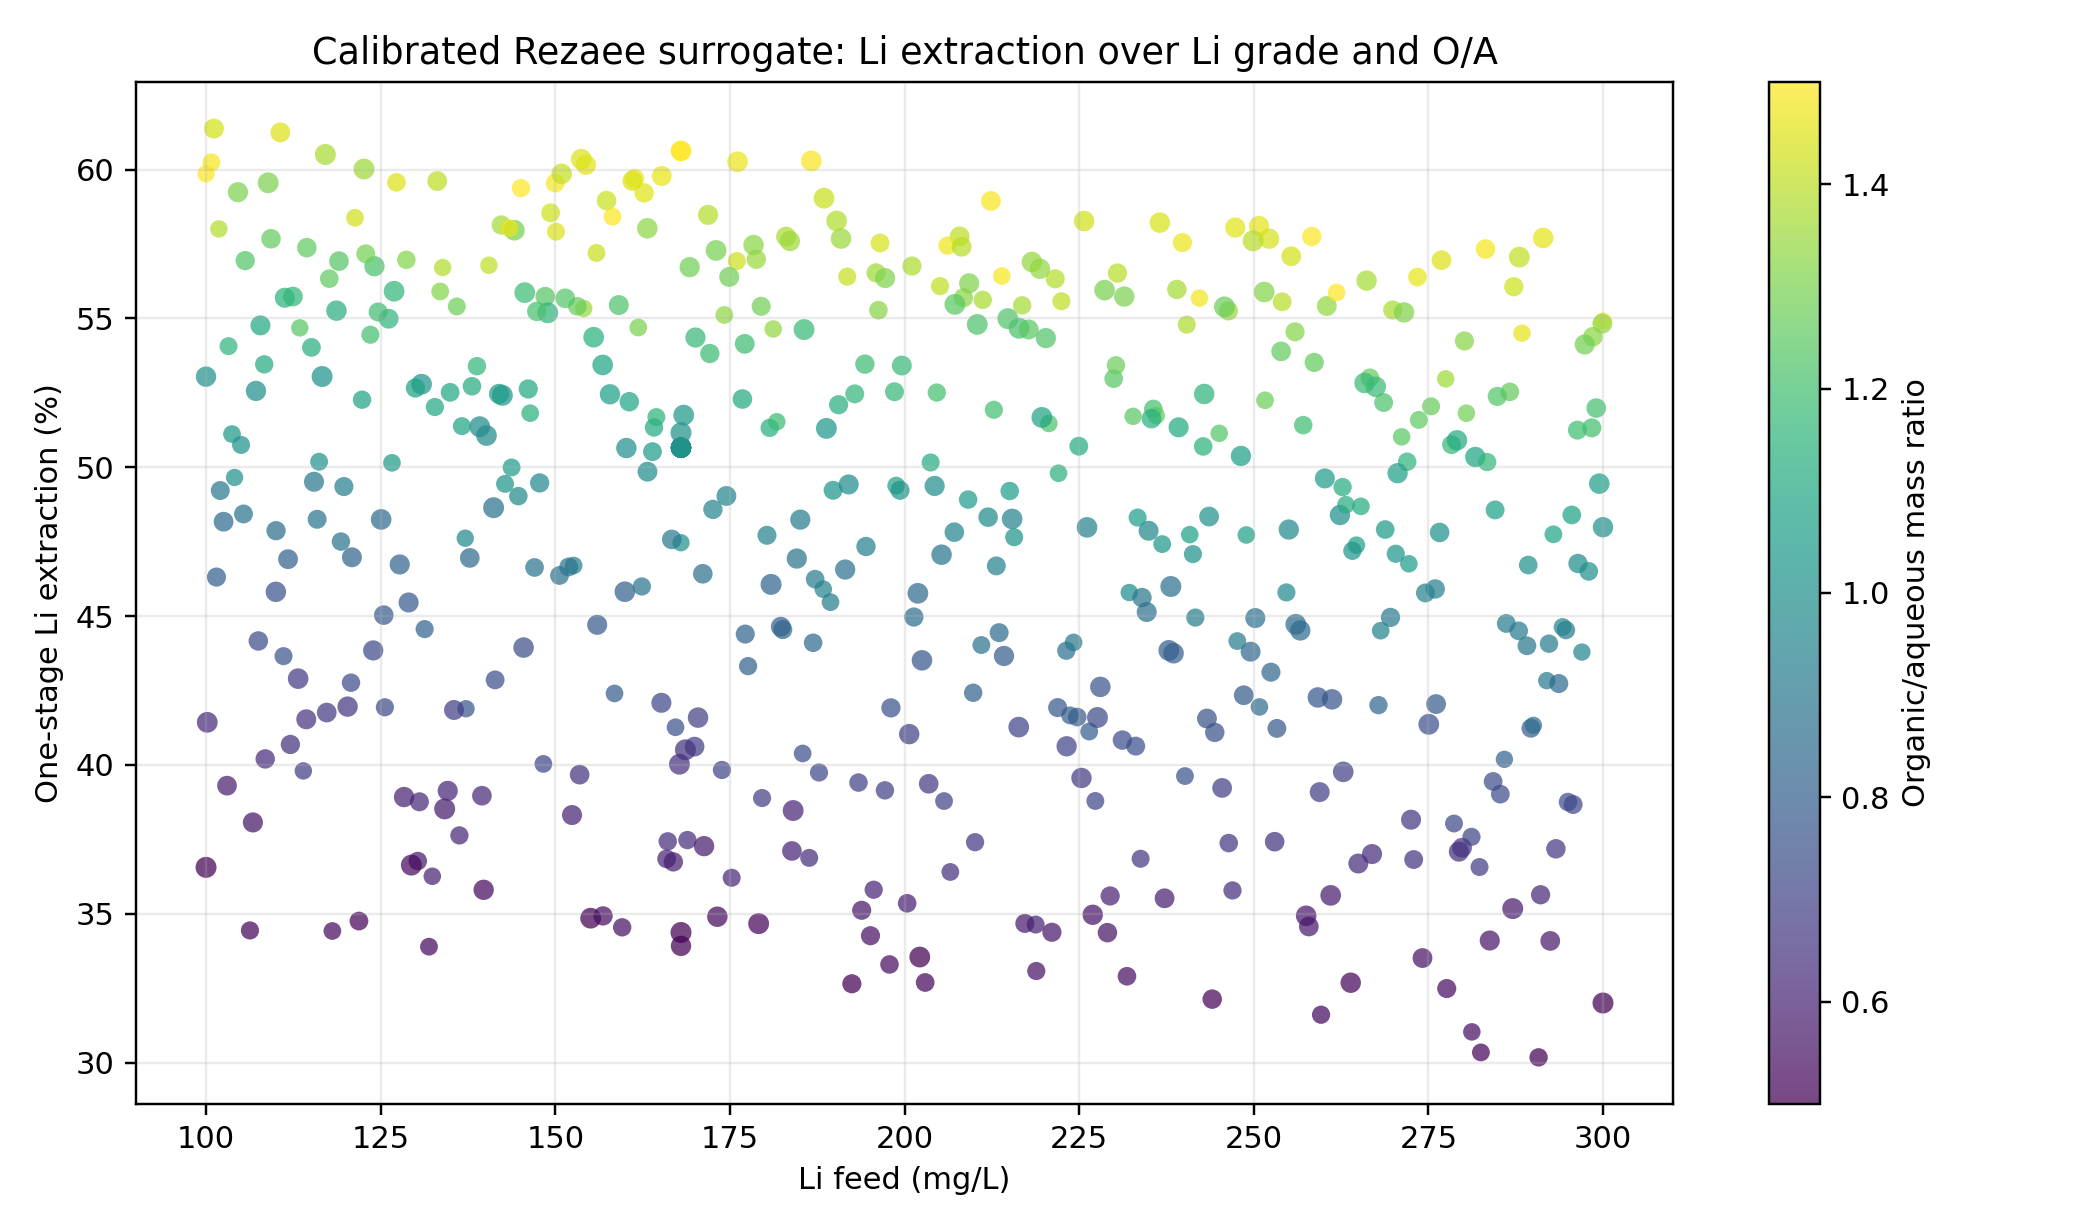
\includegraphics[width=0.78\linewidth]{calibrated_li_extraction_surface.png}
    \caption{Calibrated Rezaee surrogate lithium extraction surface over lithium feed concentration and organic-to-aqueous ratio.}
    \label{fig:li-extraction-surface}
\end{figure}

\begin{figure}
    \centering
    
\includegraphics[width=0.78\linewidth]{calibrated_selectivity_vs_na_li.png}
    \caption{Lithium-to-sodium selectivity over produced-water sodium loading. The high-\NaIon/\LiIon region is an extrapolation relative to the original Rezaee DOE space.}
    \label{fig:selectivity}
\end{figure}

The current result is most useful as an interface product: it supplies extraction, selectivity, distribution coefficients, raffinate loading, and extract loading in a form suitable for staged contactor and costing studies. It should not yet be read as an experimental guarantee for high-\NaIon/\LiIon \Smackover water.

\section{Process Handoff and Costing Scaffold}
\label{sec:process-handoff}

The \Prommis/\IDAES handoff converts the surrogate rows into a staged-contacting and cost-screening contract. The current artifacts include process-facing transfer tables and calibrated costing scenarios at a \SI{1000}{m^3/day} feed-flow basis. The screening economics use calibrated surrogate recovery values, but the costing layer remains preliminary until residence time, solvent loss, reagent make-up, pretreatment capital, product pricing, and waste handling are fixed.

\begin{figure}
    \centering
    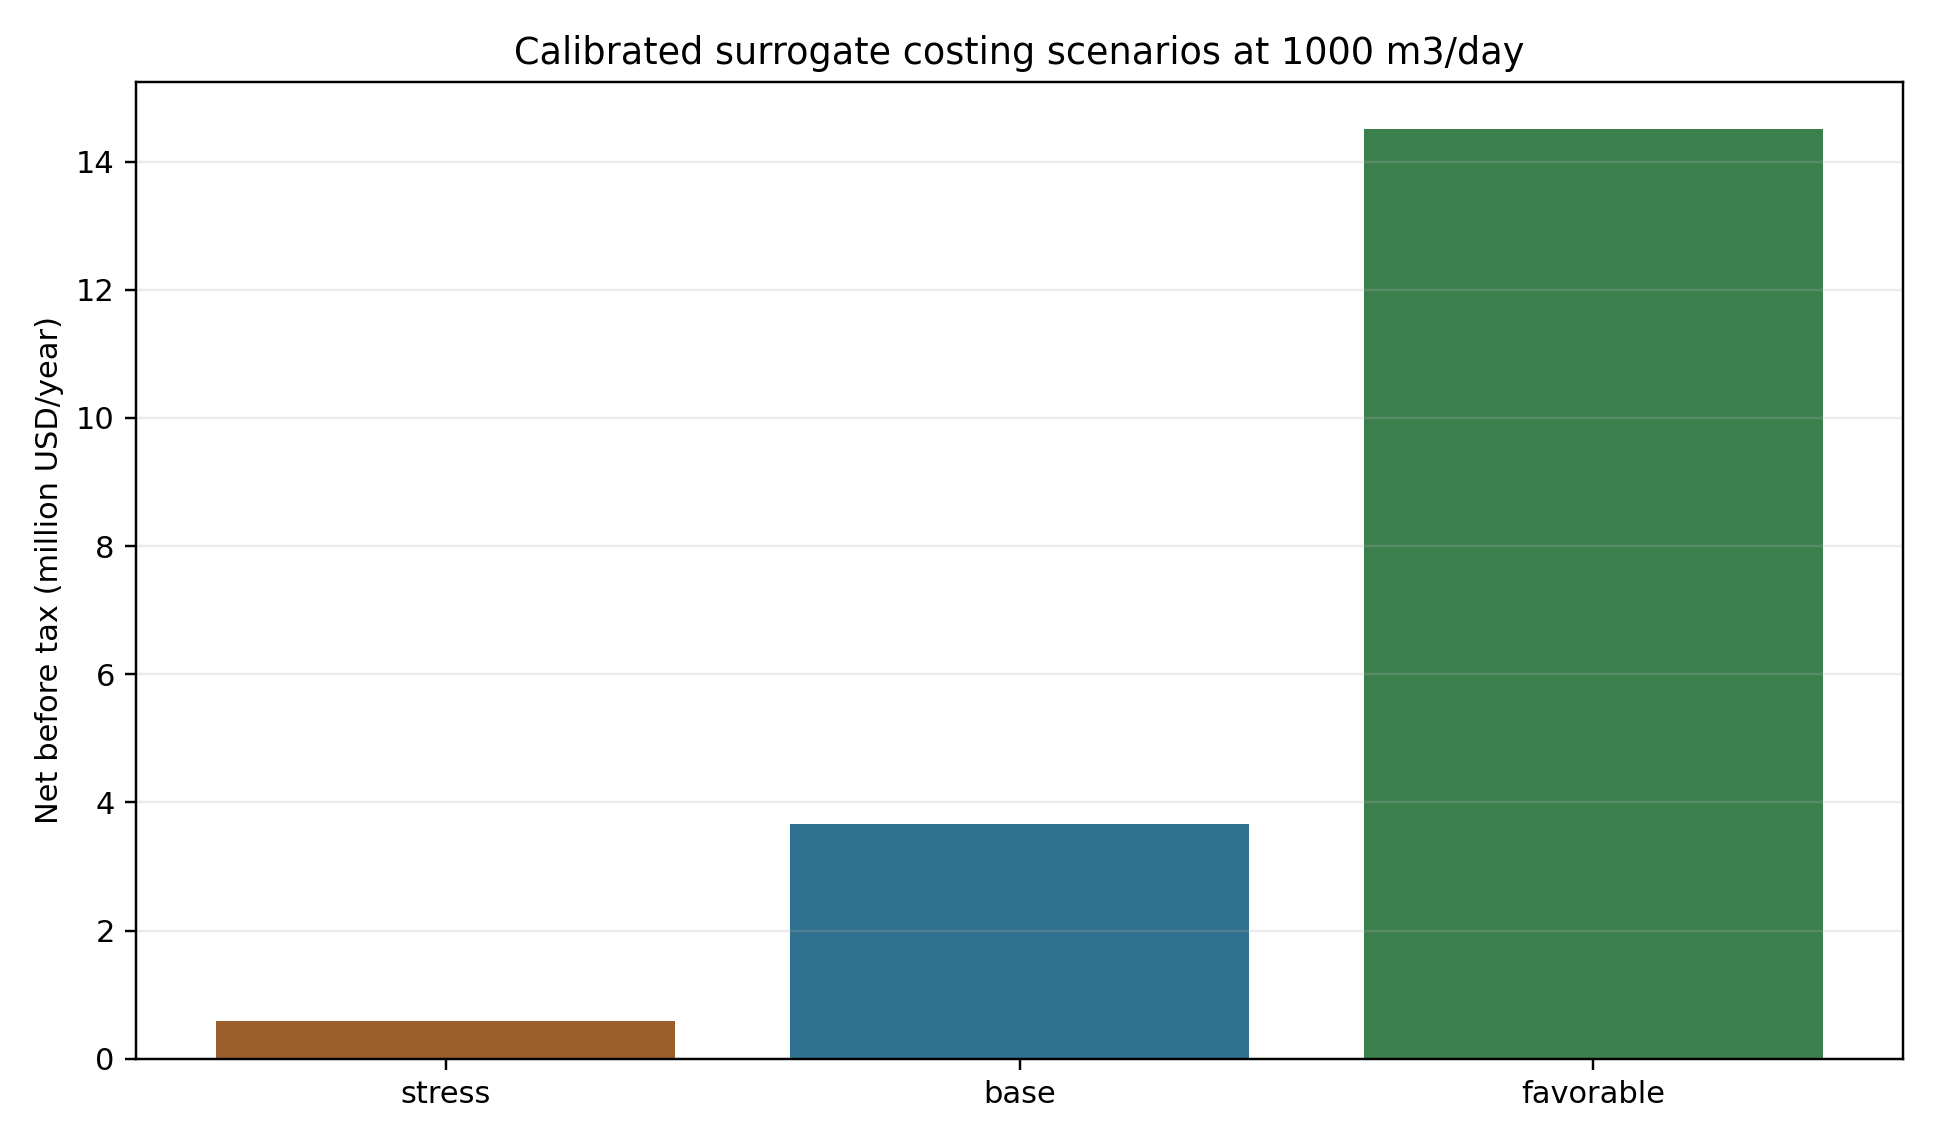
\includegraphics[width=0.78\linewidth]{calibrated_costing_scenarios.png}
    \caption{Current calibrated surrogate costing scenarios. These are screening-level economics and should be replaced by the final \Prommis/\IDAES costing block before submission.}
    \label{fig:costing-scenarios}
\end{figure}

The manuscript draft should eventually include a formal mathematical description of the staged contactor, the IDAES costing blocks, the basis for annual operating time, and sensitivity cases for solvent loss and pretreatment severity. The current version only reserves the section and records the active artifacts that must be promoted.

\section{Limitations and Next Work}
\label{sec:limitations}

The most important limitation is the sodium-load extrapolation. Every produced-water row is outside the original Rezaee DOE \NaIon/\LiIon training range, so the surrogate is currently appropriate for process screening and interface development rather than final design. A second limitation is the gap between the calibrated distribution surrogate and a fully accepted direct reactive ePC-SAFT LLE closure. The current package-facing evidence is valuable, but the manuscript should not claim an accepted physical split until the direct solve, reaction convention, and source-supported residuals are all closed.

The next paper-development steps are:
\begin{enumerate}
    \item Replace internal path references with stable citation, table, and artifact identifiers.
    \item Promote the final Rezaee regression table, residuals, and uncertainty diagnostics into the manuscript.
    \item Add the full \Prommis MSContactor equations and formal \IDAES costing assumptions.
    \item Add a transparent pretreatment model for divalent removal before the clean \LiIon/\NaIon extraction feed.
    \item Compile a final source-backed literature review covering produced-water lithium resources, hydrophobic \DES extraction, \TOPO co-extraction, and thermodynamic surrogate limits.
\end{enumerate}

\section{Conclusions}
\label{sec:conclusions}

This scaffold establishes the first manuscript structure for the produced-water lithium extraction case study. The active story is a Rezaee-calibrated \DES/\TOPO distribution surrogate applied to a pretreated \Smackover \LiIon/\NaIon stream, with explicit transfer variables for \Prommis/\IDAES process screening. The draft deliberately preserves the boundary between process-screening evidence and final predictive thermodynamics so that later revisions can strengthen the paper without overstating the current model.


\clearpage
\bibliographystyle{styles/model1-num-names}
\bibliography{references}

\end{document}
